\documentclass[a4paper, 12pt]{article}
\usepackage{comment} % enables the use of multi-line comments (\ifx \fi) 
\usepackage{lipsum} %This package just generates Lorem Ipsum filler text. 
\usepackage{fullpage} % changes the margin
\usepackage{cite}
\usepackage{graphicx}
\usepackage{wrapfig}
\linespread{1.15}
\graphicspath{ {images/} }


\begin{document}
%Header-Make sure you update this information!!!!
\noindent
\large\textbf{Carbon Storage Project} \hfill \textbf{Joshua Zweig} \\
\normalsize Carbon Storage \\
Prof. Lackner \hfill Spring 2016 \\

\begin{centering}
\textbf{Short Listing Saline Reservoirs for Potential Carbon Storage} \\
A Look at the Viability of Candidate Reservoirs in the United States through\\
Fuzzy c-Means Clustering\\
\end{centering}


\section*{Abstract}


\section{Introduction}
\subsection{Carbon Storage}
Scope to US bc available data


Motivation and whats what

\subsection{Potential Storage Site: Saline Formations}

\begin{wrapfigure}{r}{0.5\textwidth} %this figure will be at the right
    \centering
    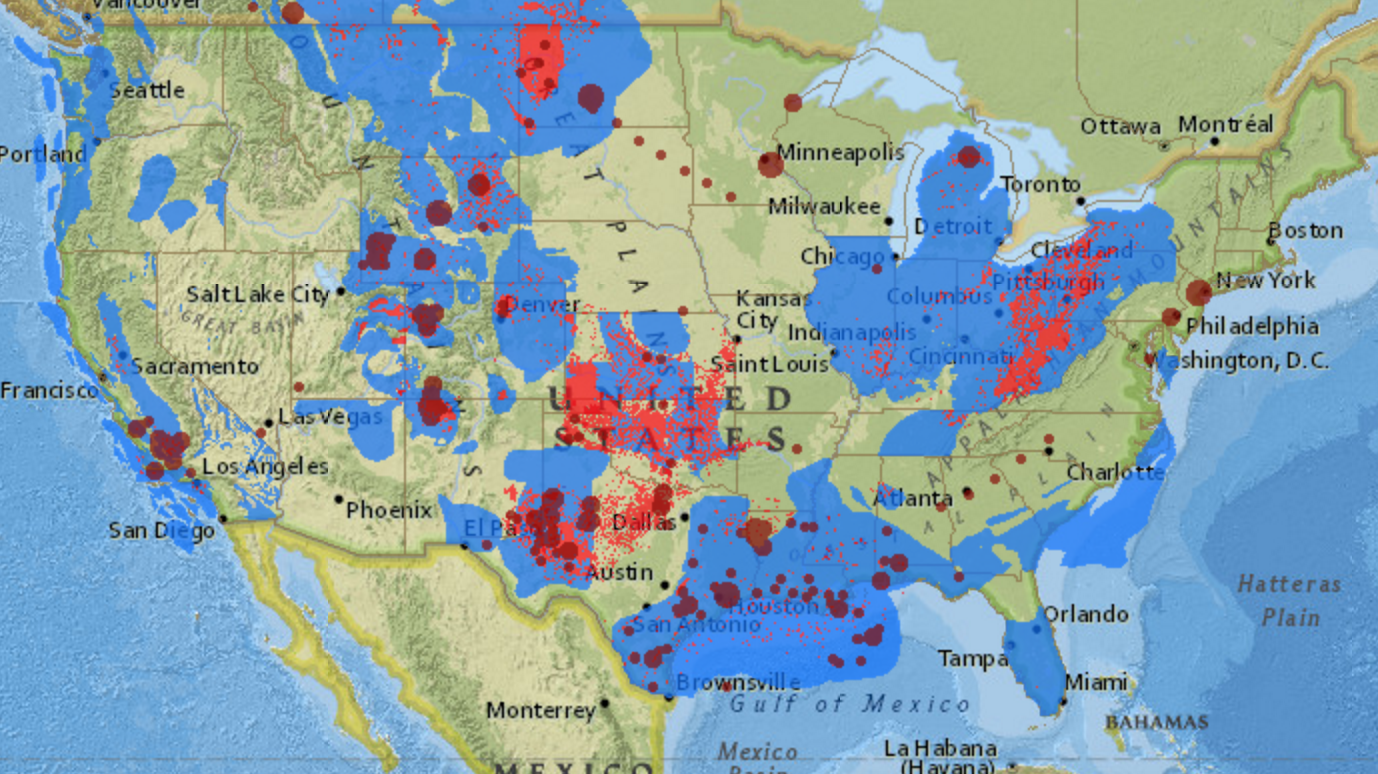
\includegraphics[width=0.5\textwidth]{saline_tight}
    \caption{\label{salinetight} A map of the United States overlaid with geological saline resources for potential carbon storage (blue), stationary sources of petroleum and natural gas (brown) and other oil and gas resources (red) \cite{atlas}}. 
\end{wrapfigure}

\par Of possible candidates for long term carbon sequestration, saline formations have emerged as a promising candidate. Such formations are prevalent throughout North America. These brine coated layers of permeable rock are able to store carbon my way of "solubility trapping, mineral trapping, structural trapping and residual trapping."

The more than 180,000 potential injection sites in the United States have been estimated by the U.S. Department of Energy to have capacity of over 12 trillion tons of CO$_2$. Saline formations are promising also because of their proximity to CO$_2$ point sources, allowing easy transition of U.S. energy assets to "near-zero carbon emissions via low-cost carbon storage retrofits." \cite{whysaline} Furthermore, there is much existing technology and regulatory acceptance with respect to injections into saline reservoirs as brines are frequently injected into saline reservoirs in EOR and the U.S. EPA has designated some deep saline formations for hazardous waste disposal.

\par There are currently at least 3 saline aquifer injection projects that have been undertaken in the continental United States, which have together injected over a million tons of CO$_2$ to date. Each of these projects operates on a time scale of at least twenty years, allocating at least 10 years to "characterizing geologic and terrestrial opportunities for carbon storage and identifying CO$_2$ stationary sources within the territories of the individual RCSPs and evaluating promising CO$_2$ storage opportunities through a series of small-scale field projects"  \cite{midwestinject}, \cite{midwestinject2}, \cite{southeastinject}. 

Important Charecterists 



\subsubsection{Associated Risk} 


\section{Methodology}
\subsection{Overview}
As described in the previous section, saline aquifers are luckily a far vast enough resource for us to currently store the desired amount of carbon. However, selecting the best aquifers for storage is a tremendous task considering the quantity of potential aquifers ($\approx180,000$) and the factors that characterize each one. For this reason we seek to develop a tool to immediately help identify some of the best candidate deep saline aquifers in the United States. 
The fundamental workings of this tool will be in the characterization of potential aquifers based on a series of characteristics as per section \ref{wellchar}. Having fully characterized each candidate aquifer, we fully employ a Fuzzy c-Means clustering analysis to each of the $\approx180,000$, 9 dimensional vectors representing the system to create a model that will determine how strongly each aquifer is characterized by each of the 9 features, to be discusses further in section \ref{fuzz}. Once this model is created, it will allow researchers to essentially filter potential storage sites by different characteristics. For example, we will be able to observe all aquifers that have at least a given storage capacity and/or are at least a given distance from a major fault line.  

\subsection{Saline Aquifer Characterization} \label{wellchar}
Each of the 9 characterization features falls into one of two categories. The first category of features describes the geological aspects of the aquifer, strictly its ability to store carbon. The second describes some of the factors that effect the potential risks and barriers to societal acceptance regarding potential storage sights. 

\subsubsection{Geological Characterization}
Natcarb

\subsubsection{non-Geological Characterization}
Other sources, check the notes.txt
The list below is a list of dimensions used to characterize saline formations with respect to environmental features not directly related to the ability of the formation to store carbon.
They are listed with reasonings for their inclusion in this early stage work in no particular order.

\begin{enumerate}
\item \emph{Potential Impact on Drinking Water Sources} 

\item \emph{Proximity to and Size of Population Centers} 

\item \emph{Proximity to and Magnitude of Fault Lines}

\item \emph{Proximity to National Parks}
\end{enumerate} 

Cover where you got your data and why you chose the features. dimensions you chose



\subsection{Fuzzy c-Means Clustering}\label{fuzz}.


\subsection{Analysis of Site Already in Use}
Talk about the few points that represent wells that are already in use and how they fit in your model. 


\section{Results}
These are some of the results

%\begin{wrapfigure}{R}{0.5\textwidth}%this figure will be at the right
  %  \centering
  %  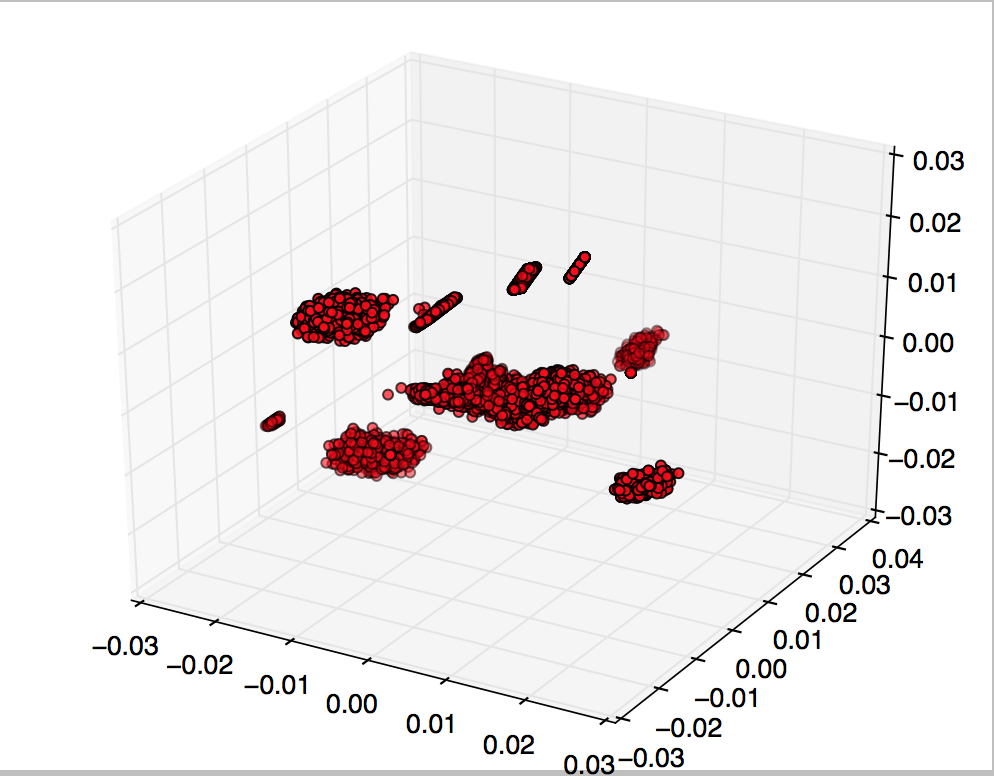
\includegraphics[width=0.5\textwidth]{clusters}
    %\caption{\label{clusters} Results of the Fuzzy c-Means clustering on the data sample}. 
%\end{wrapfigure}

%\begin{wrapfigure}{L}{0.5\textwidth}%this figure will be at the right
   %\centering
  %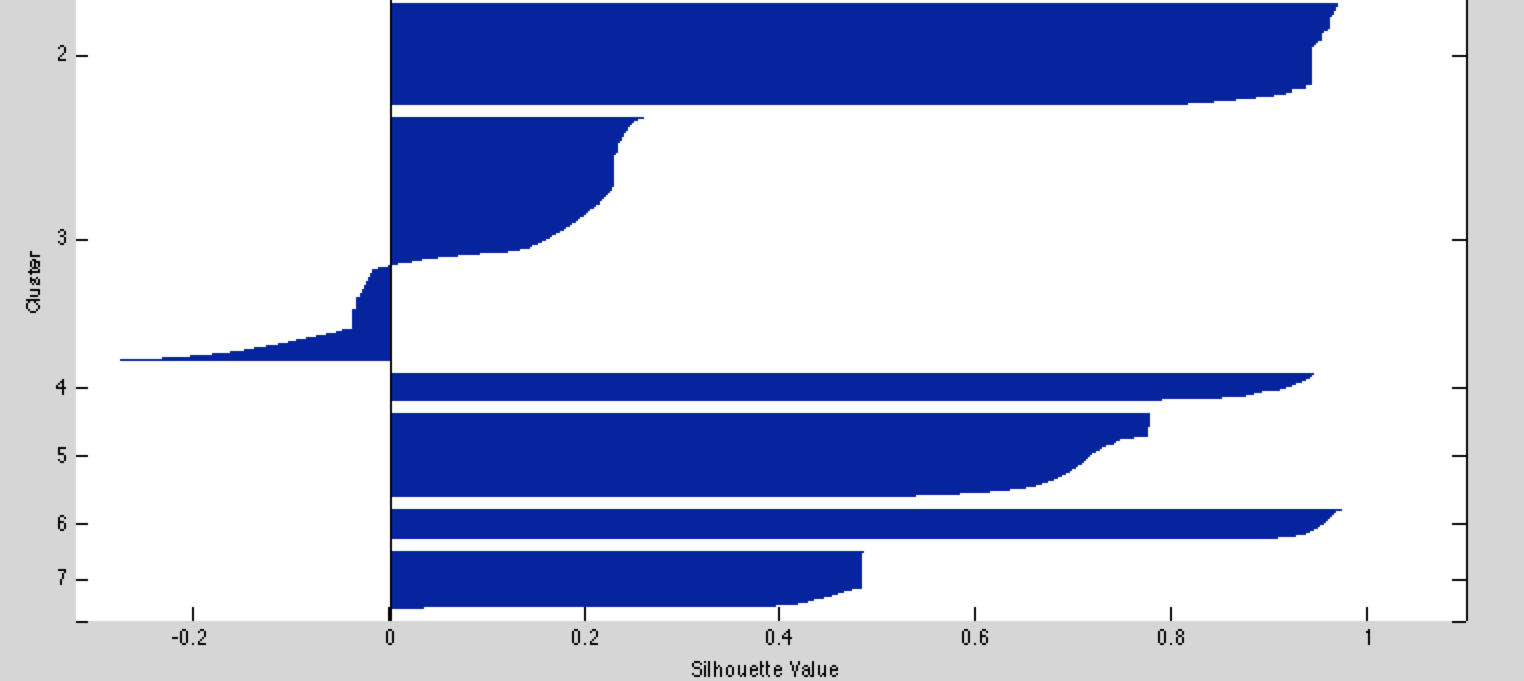
\includegraphics[width=0.5\textwidth]{k_means_sil}
  % \caption{\label{k_means_sil} ... }. 
%\end{wrapfigure}


\section{Discussion and Analysis}

\section{Future Work}
\subsection{Better Characterization of Saline Formations}
The 9 features isolated for characterization are a minimal set for reasonable characterization of saline formations. Better and more detailed (higher dimensional) characterizations of these formations would necessarily allow for more data for Fuzzy c-Means clustering to base its similarity measures on, thereby increasing the accuracy and effectiveness of this tool. Further dimensions include the existence of a caprock over the layer of porous rock. The existence of such a caprock is extremely important to the viability of a potential site as it plays an important part in keeping the injected carbon below the surface and in place.  


\section{Conclusion}

 
\begin{thebibliography}{9}

\bibitem{QuantRiskS2014}
Wriedt, J., Deo, M., Han, W. S., and Lepinski, J.
\textit{A methodology for quantifying risk and likelihood of failure for carbon dioxide injection into deep saline reservoirs}
International Journal of Greenhouse Gas Control 20 (2014), 196-211.

\bibitem{midwestinject}
Albenze, Erik, and Sallie Greenberg. 
\textit{Midwest Geological Sequestration Consortium $\|$ Development Phase}
National Energy Technology Laboratory, 1 Nov. 2015. http://www.netl.doe.gov/publications/factsheets/project/NT42588.pdf.

\bibitem{midwestinject2}
McNemar, Andrea, and Neeraj Gupta. 
\textit{Midwest Regional Carbon Sequestration Partnership $\|$ Development Phase}
National Energy Technology Laboratory, 1 Nov. 2015. http://www.netl.doe.gov/publications/factsheets/project/NT42589.pdf.

\bibitem{southeastinject}
Brown, Bruce, and Ken Nemeth. 
\textit{Southeast Regional Carbon Sequestration Partnership $\|$ Validation Phase}
National Energy Technology Laboratory, 1 Dec. 2012. http://www.netl.doe.gov/publications/factsheets/project/NT42590-P2.pdf.

\bibitem{whysaline}
\textit{Carbon Storage R\&D} Department of Energy. Office of Fossil Energy. Web. 01 May 2016.

\bibitem{atlas}
Friedmann, S. 
\textit{Carbon Storage Atlas V} 
National Energy Technology Laboratory, 1 Aug 2015.

\bibitem{PredRisk2013}
Balashov, Victor N., et al.
\textit{Predictive modeling of CO 2 sequestration in deep saline sandstone reservoirs: impacts of geochemical kinetics}
Applied geochemistry 30 (2013): 41-56.

\end{thebibliography}
\end{document}
